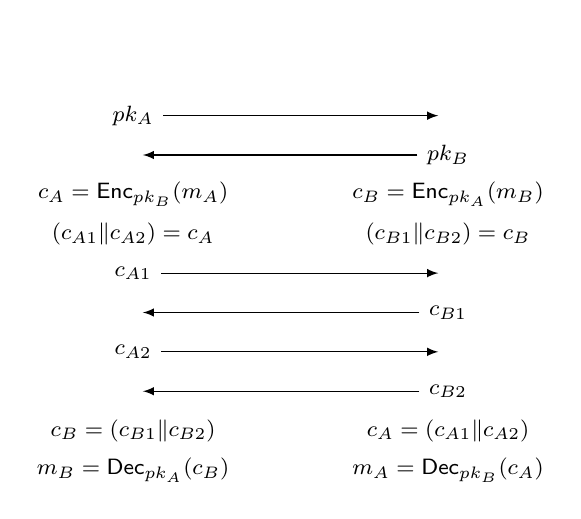
\begin{tikzpicture}[font=\footnotesize]
\node (A) at (0,0) {\Alice};
\node (B) [right of = A, node distance = 4cm] {\Bob};
\node (1a) [below of=A, node distance=1cm] {$pk_A$};
\node (1b) [below of=B, node distance=1cm] {};
\draw[-latex] (1a) -- (1b) node [midway,above] {};
\node (2a) [below of=1a, node distance=0.5cm] {};
\node (2b) [below of=1b, node distance=0.5cm] {$pk_B$};
\draw[-latex] (2b) -- (2a) node [midway,above] {};
\node (3a) [below of=2a, node distance=0.5cm] {$c_A = \mathsf{Enc}_{pk_B}(m_A)$};
\node (3b) [below of=2b, node distance=0.5cm] {$c_B = \mathsf{Enc}_{pk_A}(m_B)$};
\node (4a) [below of=3a, node distance=0.5cm] {$(c_{A1}\| c_{A2})=c_A$};
\node (4b) [below of=3b, node distance=0.5cm] {$(c_{B1}\| c_{B2})=c_B$};
\node (5a) [below of=4a, node distance=0.5cm] {$c_{A1}$};
\node (5b) [below of=4b, node distance=0.5cm] {};
\draw[-latex] (5a) -- (5b) node [midway,above] {};
\node (6a) [below of=5a, node distance=0.5cm] {};
\node (6b) [below of=5b, node distance=0.5cm] {$c_{B1}$};
\draw[-latex] (6b) -- (6a) node [midway,above] {};
\node (7a) [below of=6a, node distance=0.5cm] {$c_{A2}$};
\node (7b) [below of=6b, node distance=0.5cm] {};
\draw[-latex] (7a) -- (7b) node [midway,above] {};
\node (8a) [below of=7a, node distance=0.5cm] {};
\node (8b) [below of=7b, node distance=0.5cm] {$c_{B2}$};
\draw[-latex] (8b) -- (8a) node [midway,above] {};
\node (9a) [below of=8a, node distance=0.5cm] {$c_B = (c_{B1}\| c_{B2})$};
\node (9b) [below of=8b, node distance=0.5cm] {$c_A = (c_{A1}\| c_{A2})$};
\node (10a) [below of=9a, node distance=0.5cm] {$m_B = \mathsf{Dec}_{pk_A}(c_B)$};
\node (10b) [below of=9b, node distance=0.5cm] {$m_A = \mathsf{Dec}_{pk_B}(c_A)$};
\end{tikzpicture}
